\documentclass{Fabiano_file}
\usepackage[table,usenames,dvipsnames]{xcolor}
\usepackage{tikz} %para desenhar
\usepackage{epstopdf}
\usepackage{hhline}
\usepackage{amsmath}
\usepackage{array}
\usepackage{cancel}
\usepackage{multirow}
\usepackage{bm}
\usepackage{float}
\usepackage{makecell} % diagonal table cells
\usepackage{tabularx}
\usepackage{bold-extra} % mini caps e negrito ao mesmo tempo %
\usepackage{fixltx2e} 
\usepackage{graphicx,amssymb}
\usepackage{subcaption} 
\usepackage{alltt}
\usepackage{mathtools}
\usepackage[figuresleft]{rotating}
\usepackage{caption}
\usepackage{varwidth}
\usepackage{longtable}

\usepackage[american,cuteinductors,smartlabels]{circuitikz}
\usepackage[hidelinks]{hyperref}
\usepackage[nottoc]{tocbibind}
\usepackage[a4paper,left=2cm,right=2cm,top=2cm,bottom=3cm]{geometry}

\usepackage[export]{adjustbox}
\usepackage{graphics}
\usepackage{amssymb, amsmath, amsthm}
\usepackage{float}

\usepackage{graphicx} 
\graphicspath{{Pictures/}} 
\usepackage{eso-pic}

\setcounter{secnumdepth}{5}

\usepackage{listings}
\usepackage{color}    %May be necessary if you want to color links
\usepackage{hyperref}
\hypersetup{
    colorlinks=true, %set true if you want colored links
    linktoc=all,     %set to all if you want both sections and subsections linked
    linkcolor=blue,  %choose some color if you want links to stand out
}
\lstset{language=C}

\usepackage{background}
\backgroundsetup{
scale=1,
angle=0,
opacity=.1,  %% adjust
contents={\includegraphics[width=\paperwidth,height=\paperheight]{Electronics-Application}}
}

\title{Projeto PCB do Projeto Motor de Passo.\\Trabalho Baseado no Artigo:\\2010-Application of Proteus Virtual System Modelling (VSM) in Teaching of Microcontroller }
\author{Aluno: Fabiano Aparecido Marino \\NºUsp:7143980}

\begin{document}
{

	\newpage
	\thispagestyle{empty}
	\clearpage
	\begin{sidewaysfigure}[ht!]
		\centering
		\includegraphics[width=700pt]{CAPAC}
	\end{sidewaysfigure}
	\clearpage
	\pagenumbering{arabic}
	\newpage

\maketitle

\begin{figure}[h!]
\centering
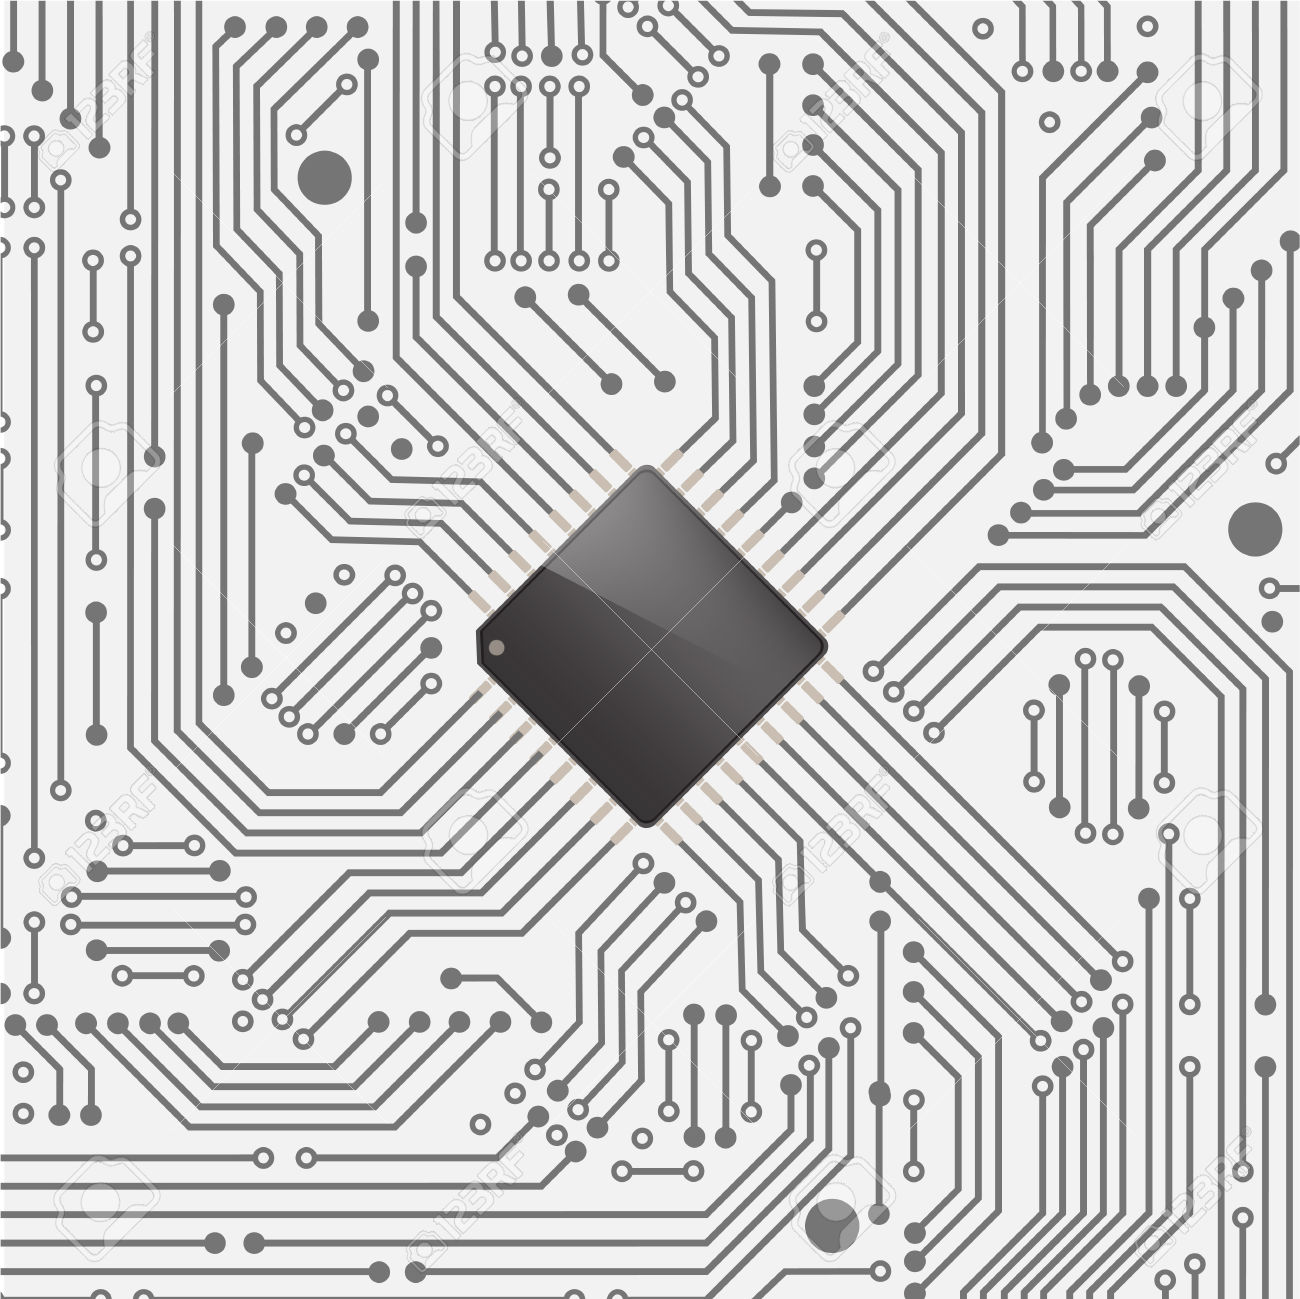
\includegraphics[width=.9\textwidth]{capa.jpg}
\end{figure}

\newpage

\tableofcontents
\listoffigures
\newpage

\section{Introdução aos Projetos PCB}
A vantagem VSM é Permitir a  prévia simulação do projeto, incluindo esquemático e software, para assim partir para a montagem PCB do projeto em questão.
Como há diversos projetos simulados no material 80c51 ISIS, pode-se modficá-los de modo a torná-los pronto para a confecção PCB.\\
A simulação não exige, por exemplo, que seja colocado o crystal oscilador no micro, oque é essencial na construção.Outro fato é que ligações com o meio externo
a placa exige que seja colocado conectores, que permitam que comunicação usada seja implementada na prática.\\
Outro fator é a presença de fonte de tensão para alimentar os dispositivos que necessitam de alimetação, sendo o micro um deles.Não será focado em como 
construir a fonte, mas sim será utilizada no projeto em questão.Outro fato é que nem todos os pinos do micro aparece no esquemático, sendo os pinos ocultos o
VCC e GND, para que no PCB o micro fique alimentado, basta colocar um probe de 5 Volts ligado ao 5 volts gerado pela fonte e um probe de 0 volts no terminal de terra
da fonte, porém isto depois de simular o sistema sem nenhum dos probes de alimentação, somente com os provindo da fonte.\\
O projeto a ser simulado e posteriormente construído neste documento encontra-se na figura abaixo que toma a página inteira, que consiste no micro 80c51 junto ao driver do motor 
de passo e fonte.Para melhor aproveitamento dos recursos disponíveis no 80c51 serão adicionados conectores que permitem posterior uso das portas que ficaram
sobrando, além do uso de um chip MAX232 que possibilita a comunicação serial com o meio externo, havendo uma forma de interface homem máquina.\\
Os componentes necessários para a construção do esquemático do motor de passo encontra-sena lista de materiais abaixo na figura abaixo.O programa que permite a
simulação do esquemático proposto encontra-se no apêndice.

\begin{figure}[h!]
\centering
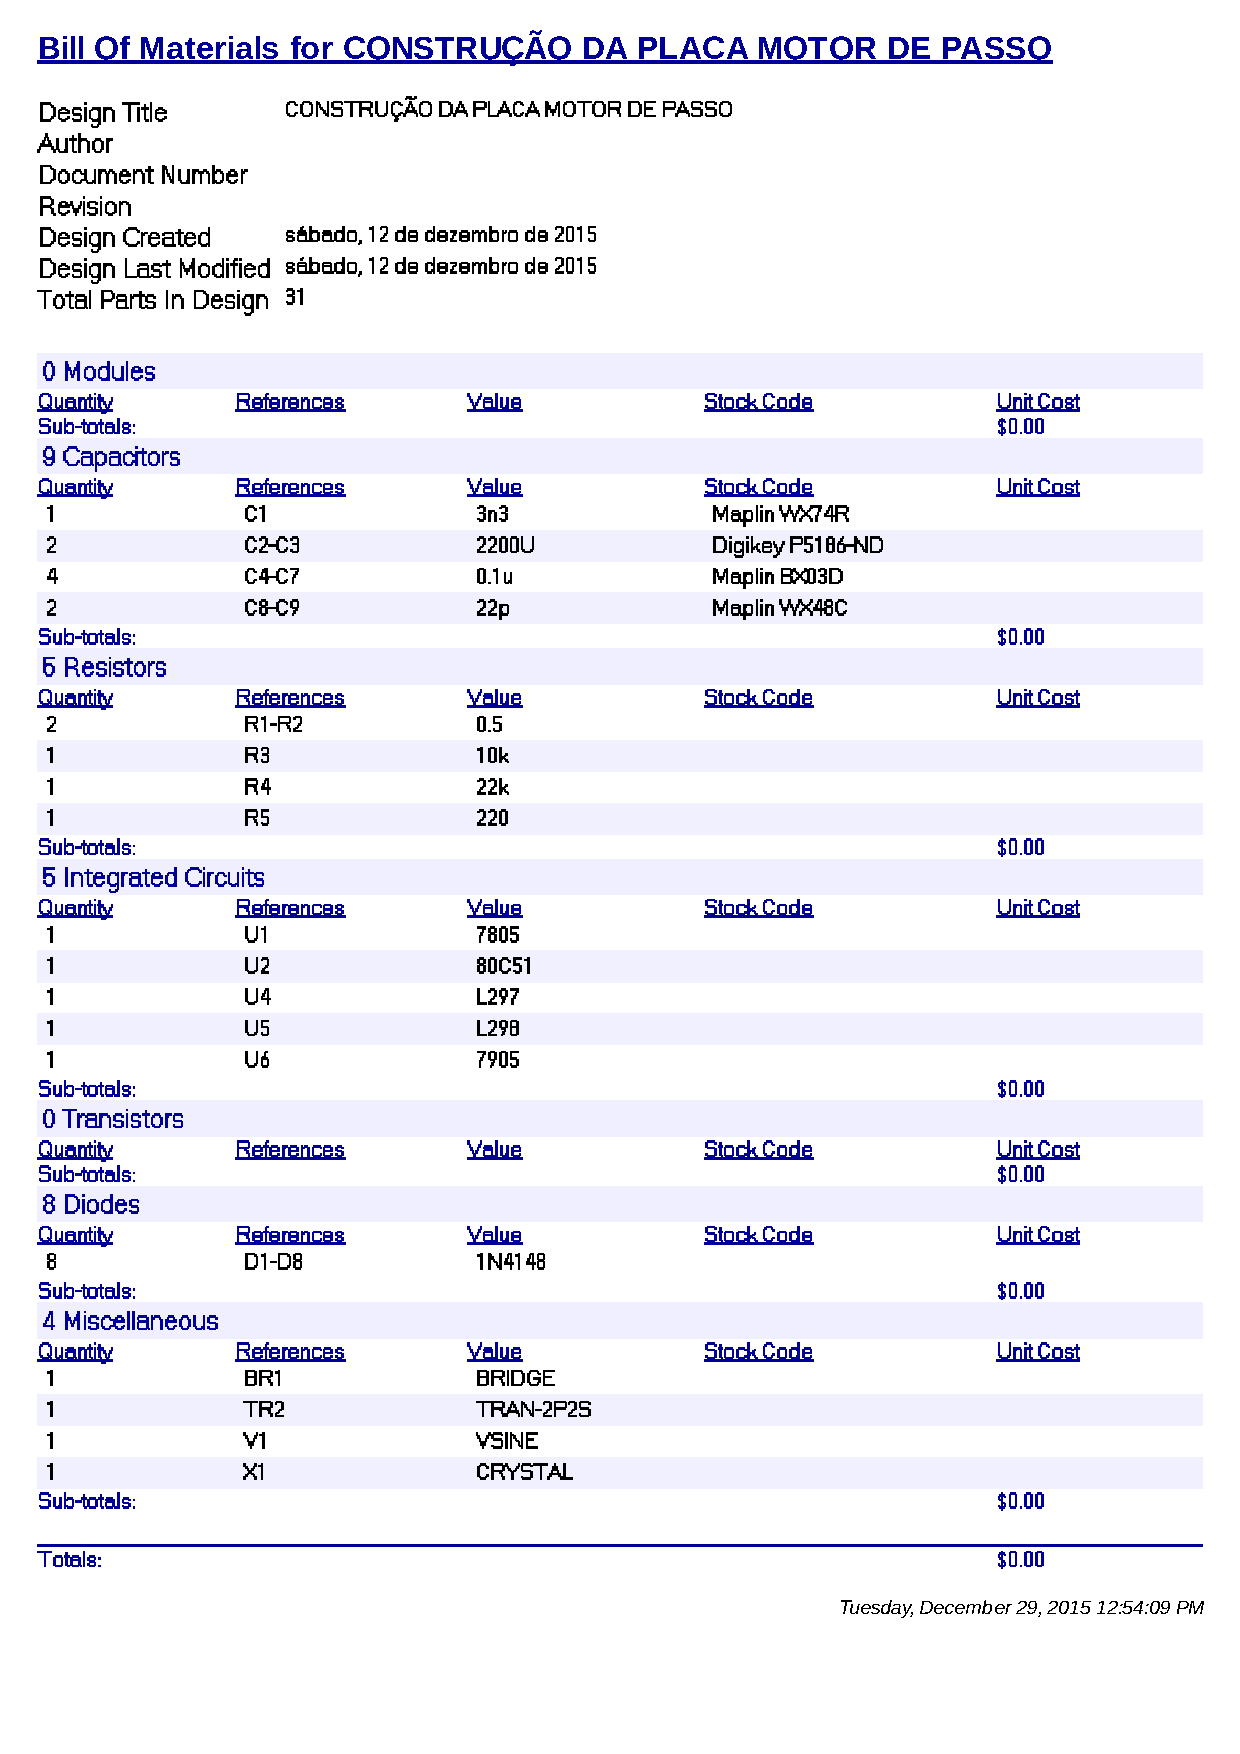
\includegraphics[width=.5\textwidth]{lista_de_materiais.pdf}
\caption{Lista de Materiais Para Construção do Esquemático do Motor de Passo}
\label{fig:lista_de_materiais}
\end{figure}

	\newpage
	%\thispagestyle{empty}
	\clearpage
	\begin{sidewaysfigure}
		\centering
		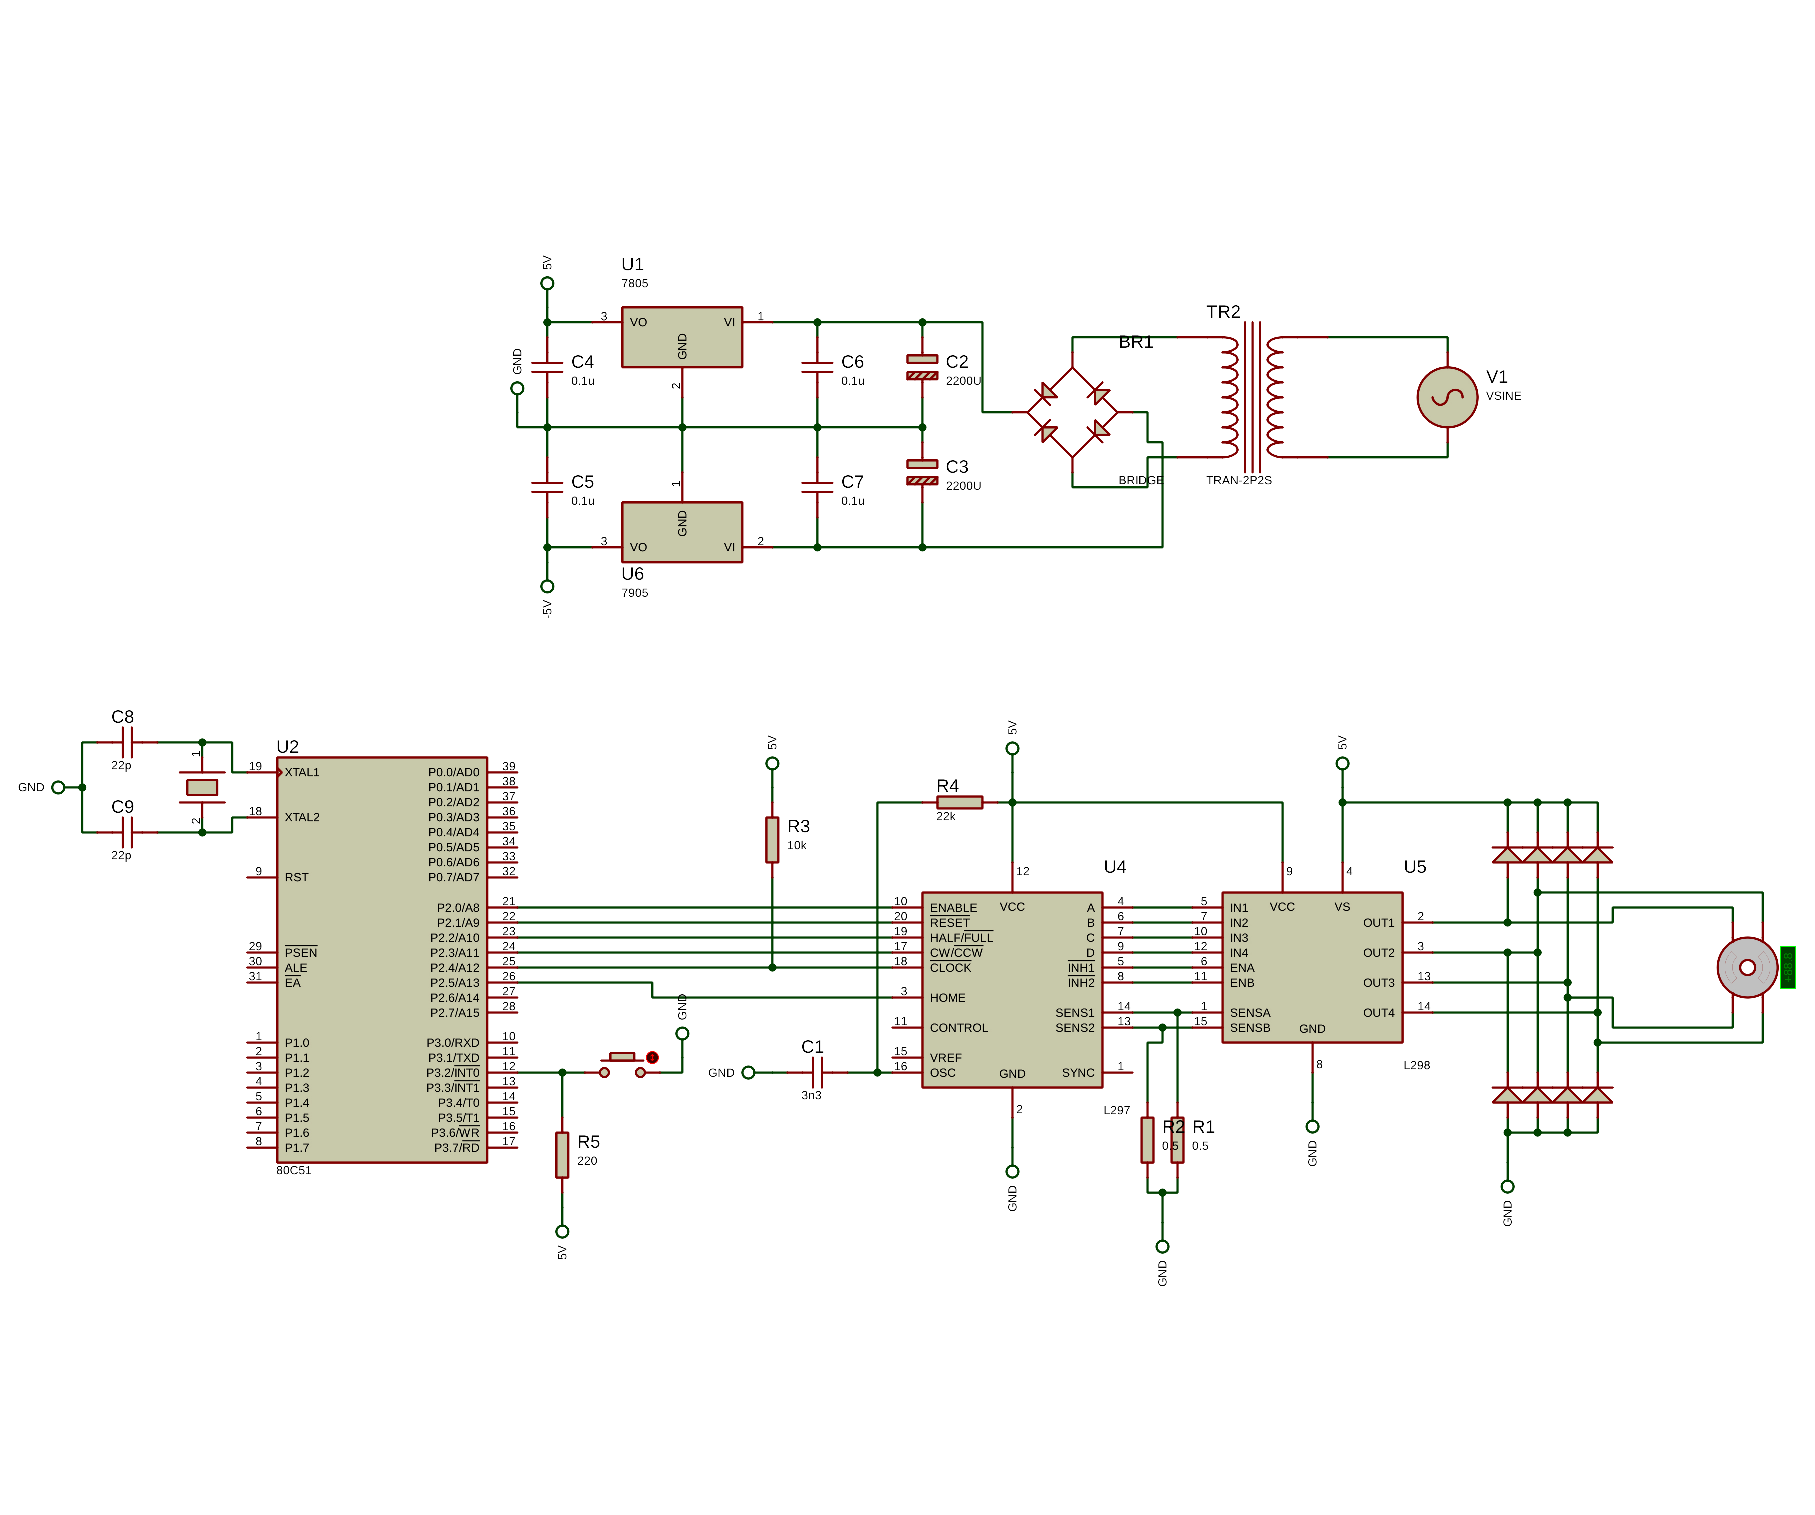
\includegraphics[width=.9\linewidth]{esquematico_do_motor_de_passo_para_simulacao}
		\caption{Esquamático Para Simulação}
	\end{sidewaysfigure}
	\clearpage
	%\pagenumbering{gobble}
	\newpage
	
\section{Montagem do Esquemático Para a Confecção PCB}
Como foi dito, para aproveitar todos os oferecimentos do micro, pelo menos ao máximo que puder no presente projeto, é preciso adicionar conectores que possibilitam
posterior uso das portas que sobraram e implemetar o uso da serial no protocolo RS232, oque exige o uso do componente MAX232.Os conectores utilizados chama-se SIL
e são oferecidos em vários números de conexões, desde uma conexão até várias, cobrindo também 8 conexões para uma porta inteira.O botão no esquemático do motor
de passo representa o momento em que ocorre a interrupção, assim o mesmo será trocado por um conector sil também.A porta serial precisa de um conector COMPIM, que 
devem ser adicionados no projeto.\\
Na próxima figura de página inteira encontra-se o esquemático pronto para construção, contando ainda com a possibilidade de interface serial.Logoa abaixo encontra-se
a lista de materiais necessárias para a confecção do esquemático.

\begin{figure}[h!]
\centering
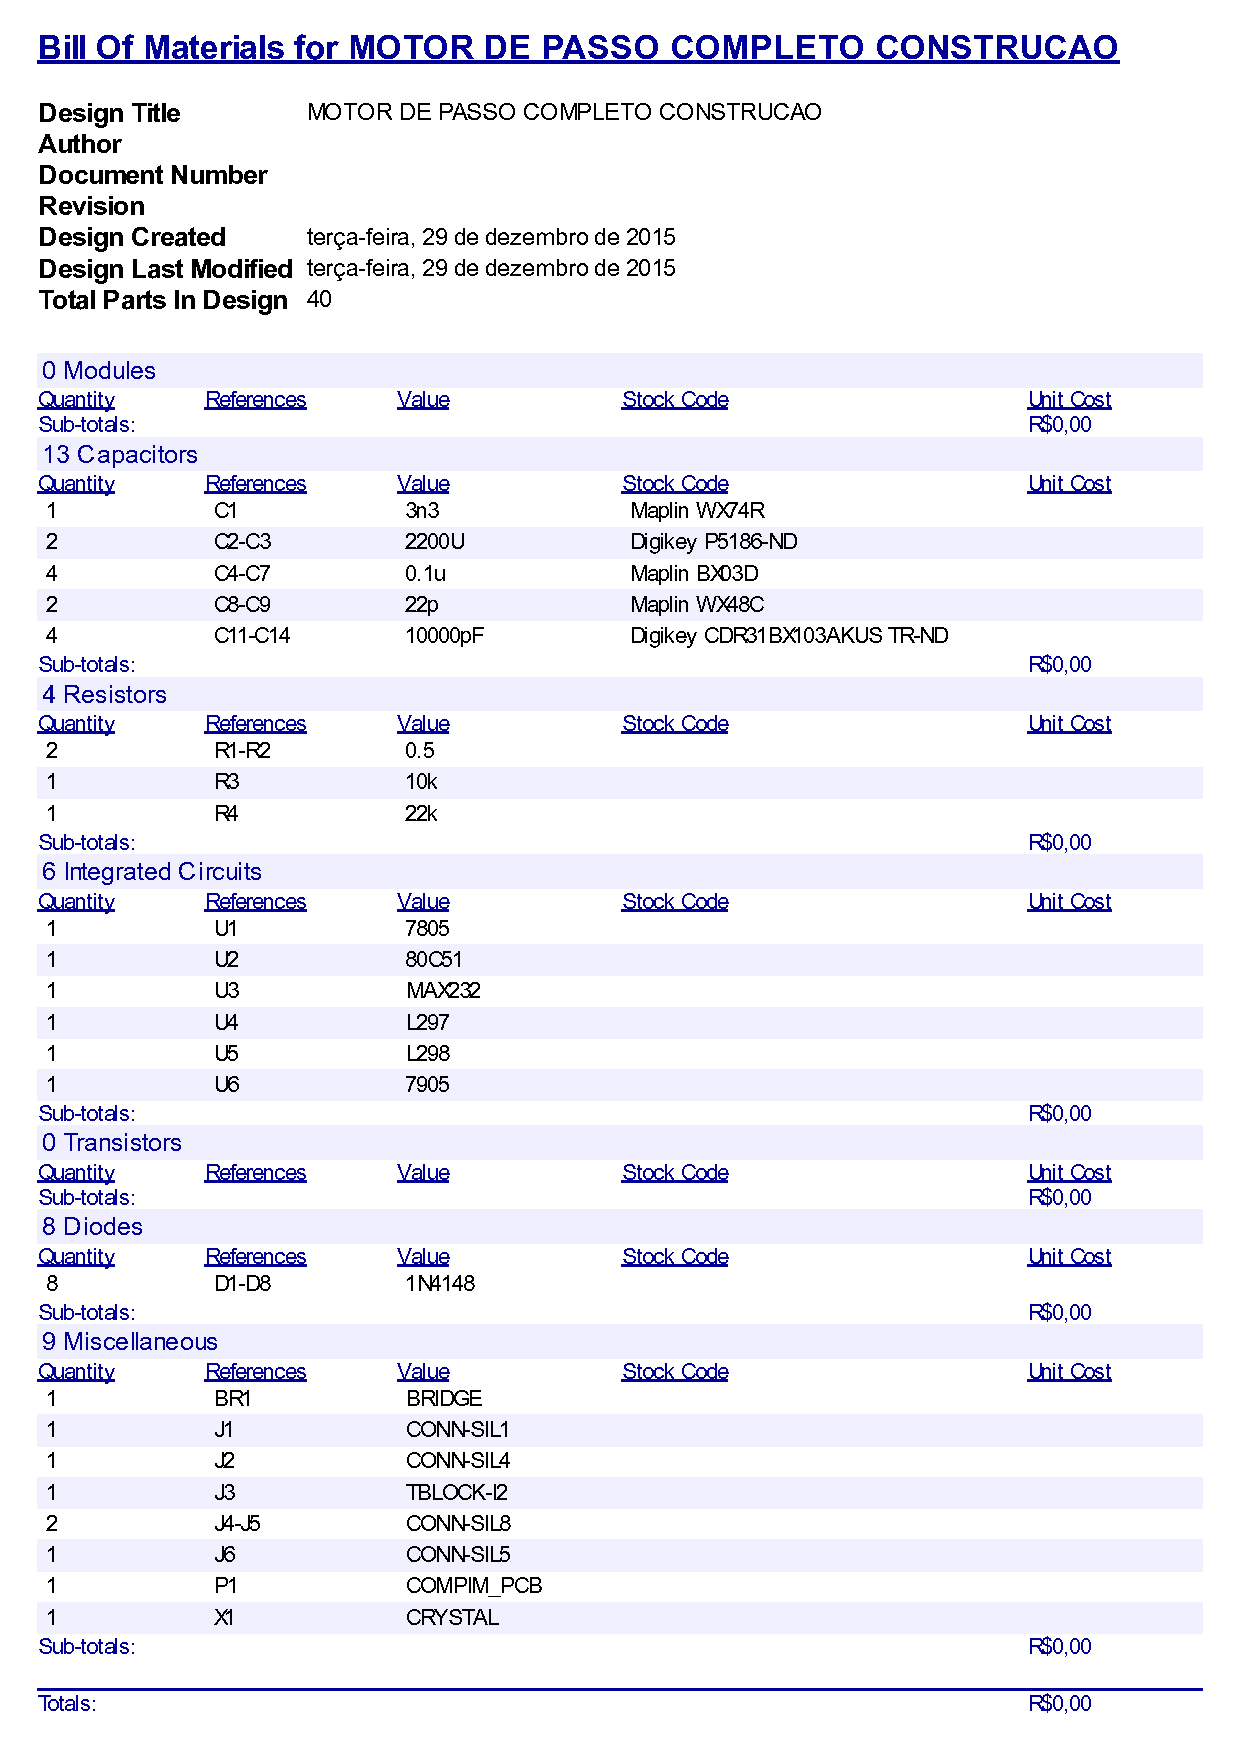
\includegraphics[width=.7\textwidth]{lista_de_materiais_completa.pdf}
\caption{Lista de Materiais Para Construção do Esquemático do Motor de Passo Completo}
\label{fig:lista_de_materiais}
\end{figure}

	\newpage
	%\thispagestyle{empty}
	\clearpage
	\begin{sidewaysfigure}
		\centering
		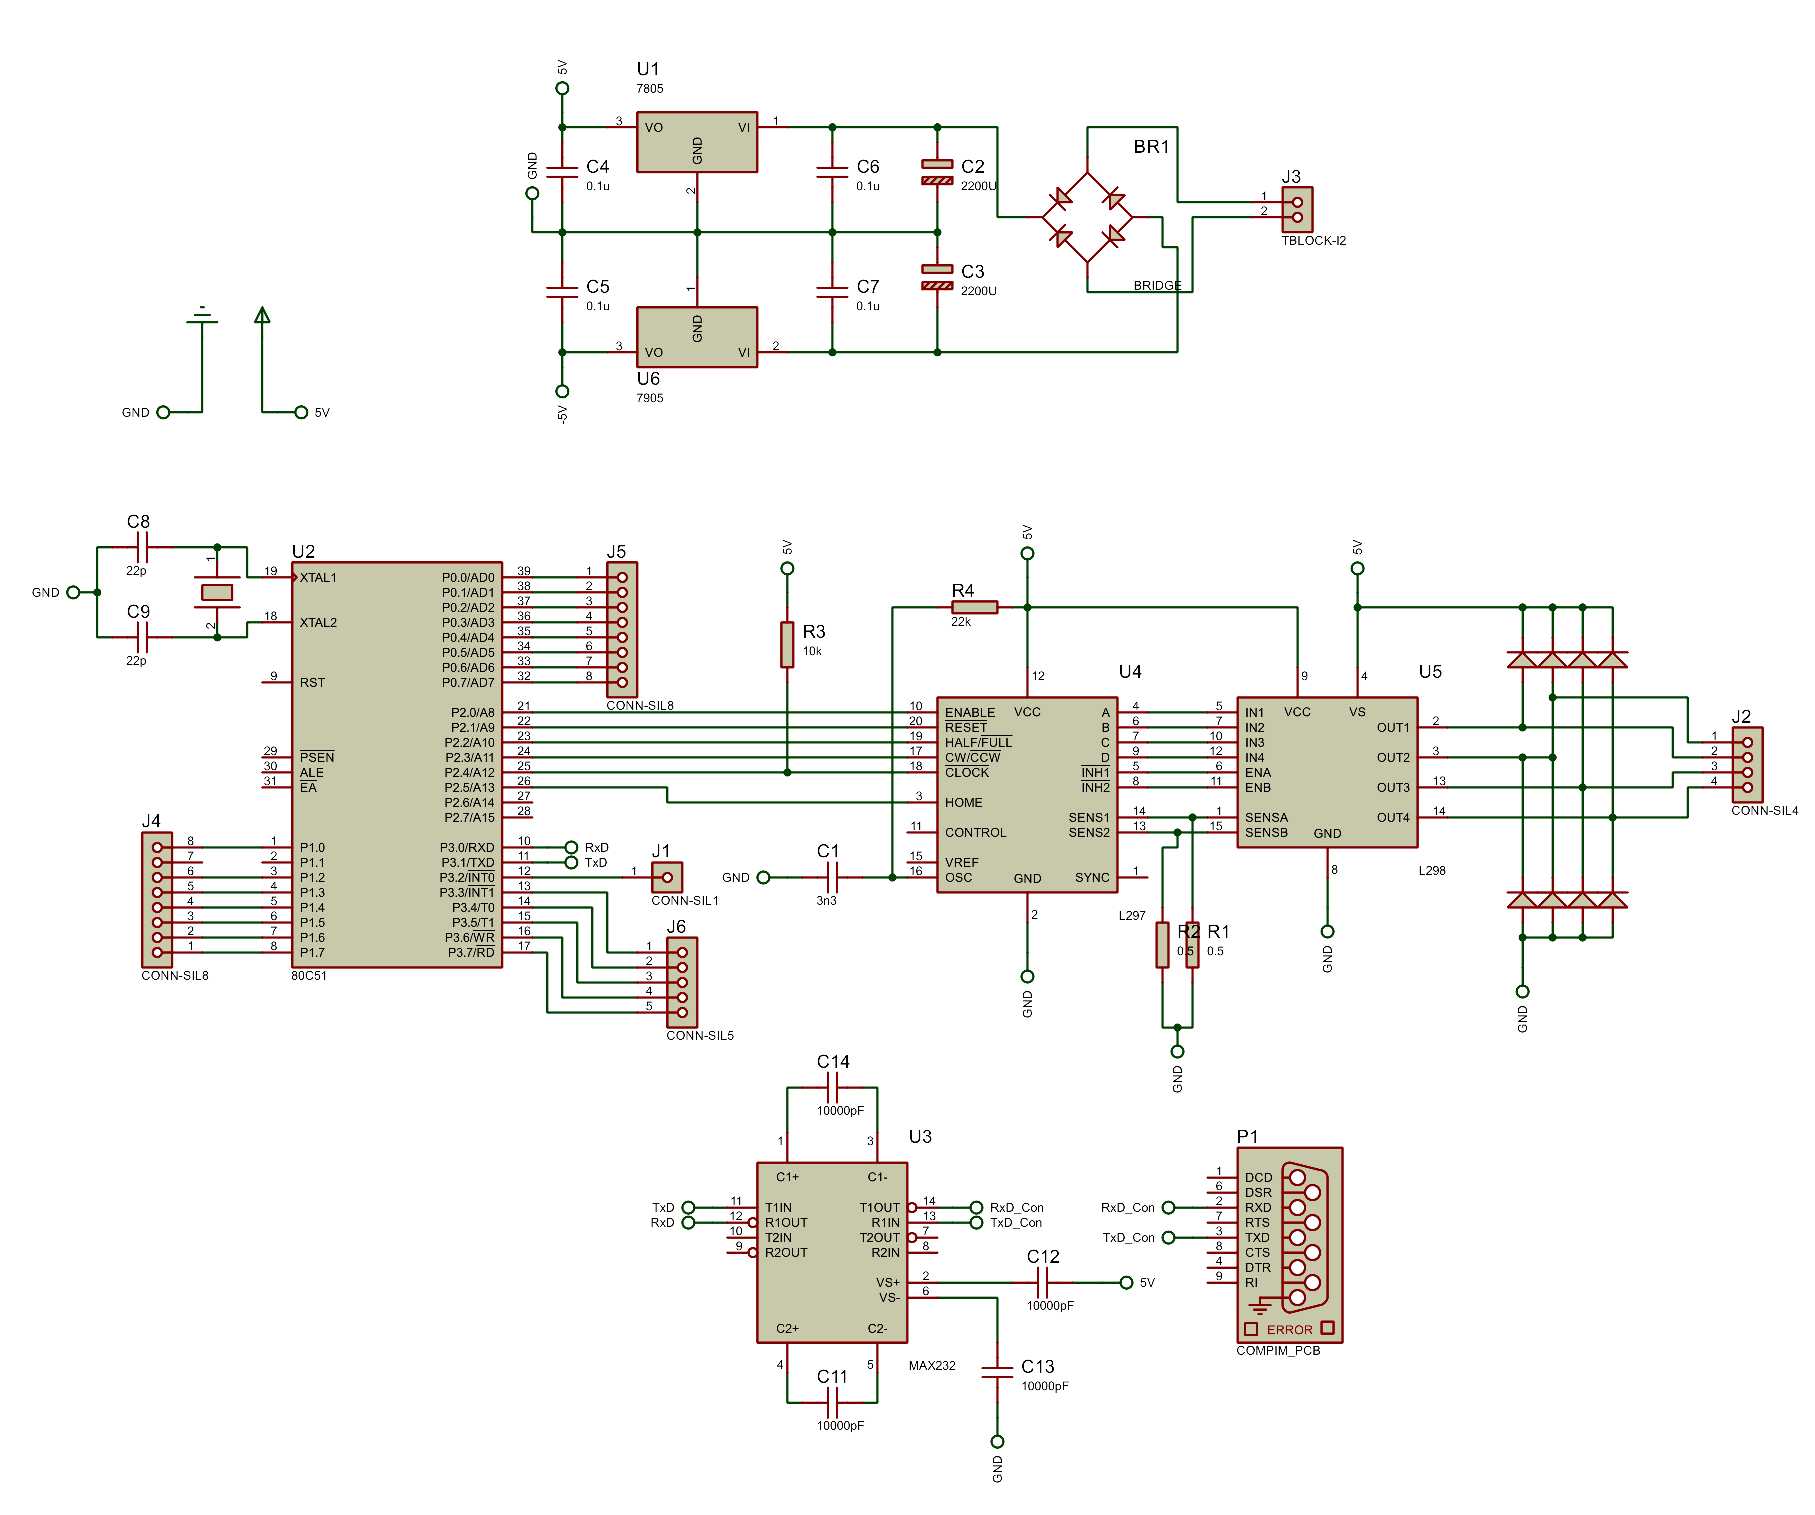
\includegraphics[width=.9\linewidth]{esquematico_pronto_para_construcao}
		\caption{Esquemático Pronto Para a Construção}
	\end{sidewaysfigure}
	\clearpage
	%\pagenumbering{gobble}
	\newpage

\section{Ares}
Tendo o esquemático pronto para confecção pronto, basta transportá-lo para a plataforma ARES, lembrando que o proteus é constituído pela plataforma ISIS, aonde 
monta-se o esquemático, e a plataforma ARES, aonde constroe-se o PCB.Ambas as plataformas são parecidas, mudando o fato de que o plano de fundo default é preto,
e que no lugar aonde estavam os componentes escolhidos ficam os componentes que foram transportados para o ARES.Para iniciar a montagem do PCB basta ir seguindo
o esquemático e clicando sobre o componente correspondente no ARES posteriormente alocando-o na posição desejada.Há poucas regras quanto a confecção de PCB, uma 
delas é que o crystal oscilador, junto aos capacitores, devem ficar próximos aos pinos de alimentação do clock do micro.Não deixar os componentes próximos no 
esquemático distantes no PCB também é um erro, frizando o fato de que deve-se seguir o esquemático para a construção do PCB.\\
Abaixo encontra-se uma figura com o PCB montado expressando a distribuição dos componentes, sempre seguindo o esquemático.

\begin{figure}[h!]
\centering
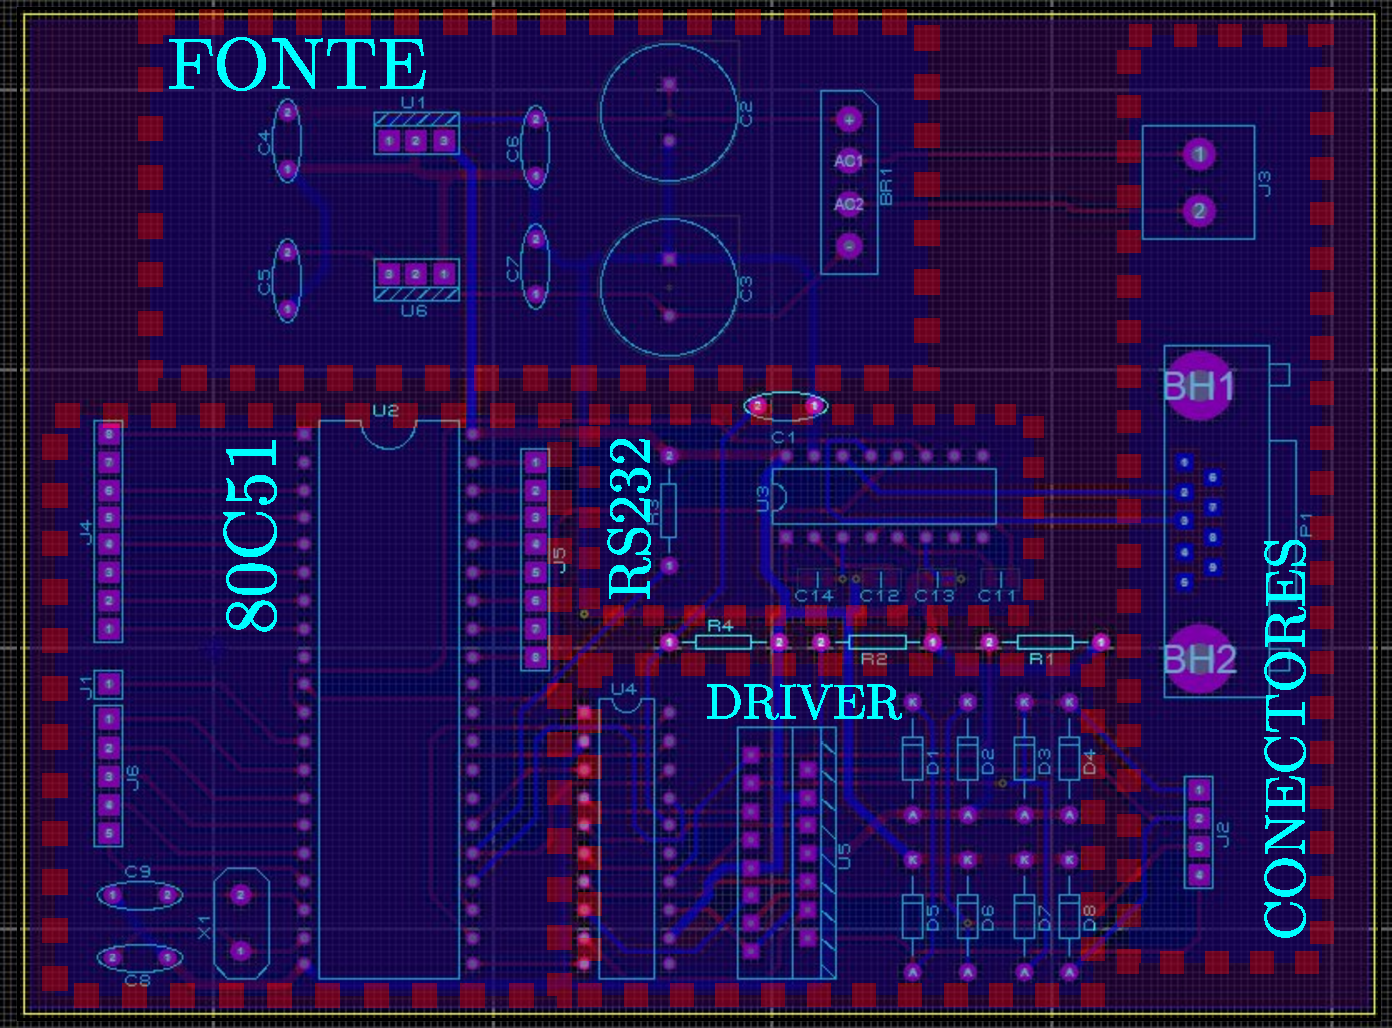
\includegraphics[width=1\textwidth]{projeto_pcb_com_rotulos.pdf}
\caption{PCB com Indicações do Posicionamento de Cada Bloco de Execução}
\label{fig:lista_de_materiais}
\end{figure}

\newpage

Por fim fica a possibilidade de se realizar a renderização da placa afim de fazer reajustes finais, isto é possível clicando em visualização 3D.Abaixo encontra-se
a imagem gerada para a placa em questão.\\
Roteamento e largura de trilhas também são fatores importantes, porém exigi-se, para completa e precisa confecção do prjeto, conhecimento de características de 
potência do projeto.Como não há esse tipo de informação fica a disposição do projetista especificar a largura das trilhas e outras configurações para verificar
as mudanças ocorridas no projeto.

\begin{figure}[h!]
\centering
\includegraphics[width=1\textwidth]{render_pcb.pdf}
\caption{Placa Renderizada Pronta}
\label{fig:render_pcb}
\end{figure}

\newpage

\section{Apêndice:Programa para Simulação do Motor de Passo}
\begin{lstlisting}
 ORG 0000H;
	SJMP INICIO;

	ORG 0003H
	CPL INT;
	CLR SENTIDO;
	RETI;

	ORG 001BH;
	CPL CLOCK;
	MOV TH1,#88H;
	MOV TL1,#01H;
	RETI;
	
ENABLE   EQU P2.0;
RESET1   EQU P2.1;
HALFULL  EQU P2.2;
SENTIDO  EQU P2.3;	
CLOCK    EQU P2.4;
HOME     EQU P2.5;
INT      EQU 20H.1;

INICIO: 
	LCALL INTERRUPT_CONFIG;
	LCALL TIMER_CONFIG;
	SETB ENABLE;
	SETB RESET1;
	CLR HALFULL;
	CLR SENTIDO;   	
	CLR HOME;
	CLR INT;
	JNB INT,$;
	CLR ET1;
	CLR ENABLE;
	LCALL DELAY5S;

	MOV TH1,#88H;
	MOV TL1,#01H;

	SETB ET1;	
	SETB SENTIDO;
	SETB ENABLE;
	JB INT,$;
	CLR ENABLE;
	CLR ET1;
	LCALL DELAY10S;

	MOV TH1,#88H;
	MOV TL1,#01H;

	SETB ET1;
	SJMP INICIO;
	
INTERRUPT_CONFIG:
	SETB EA;		
	SETB ET1;		
	SETB EX0;		
	SETB IT0;		
	RET;

TIMER_CONFIG:
	MOV TH1,#88H;
	MOV TL1,#01H;
	SETB TR1;
	RET;


DELAY5S:
	MOV	R3, #002h
	MOV	R2, #08Ah
	MOV	R1, #06Ch
	MOV	R0, #04Bh
	NOP
	DJNZ	R0, $
	DJNZ	R1, $-5
	DJNZ	R2, $-9
	DJNZ	R3, $-13
	MOV	R1, #02Fh
	MOV	R0, #0B0h
	NOP
	DJNZ	R0, $
	DJNZ	R1, $-5
	RET;

DELAY10S:
		MOV	R4, #004h
	MOV	R3, #0A0h
	MOV	R2, #002h
	MOV	R1, #018h
	MOV	R0, #093h
	NOP
	DJNZ	R0, $
	DJNZ	R1, $-5
	DJNZ	R2, $-9
	DJNZ	R3, $-13
	DJNZ	R4, $-17
	MOV	R2, #00Fh
	MOV	R1, #0B2h
	MOV	R0, #008h
	NOP
	DJNZ	R0, $
	DJNZ	R1, $-5
	DJNZ	R2, $-9
	MOV	R1, #005h
	MOV	R0, #0DCh
	NOP
	DJNZ	R0, $
	DJNZ	R1, $-5
	RET;
	
	END;
\end{lstlisting}


\end{document}
